%todo seitenumbruch \newpage

\documentclass[pdftex,12pt,a4paper]{article}
%\documentclass[a4paper,10pt]{article}
\usepackage{listings}
\usepackage[pdftex]{graphicx}
\usepackage{graphicx}
\usepackage{amsmath}
\usepackage[svgnames]{xcolor}
\newcommand{\HRule}{\rule{\linewidth}{0.5mm}}
\lstset{language=python}
\usepackage{caption} %zeilenumbruch praktisch ueberall moeglich

\parindent 0pt

\definecolor{lightpurple}{rgb}{1,1,1}
 
\lstset{
numbers=left,
stepnumber=1,
numbersep=5pt,
numberstyle=\small\color{black},
basicstyle=\ttfamily,
keywordstyle=\color{blue},
commentstyle=\color{Green},
stringstyle=\color{red},
frame=single,
tabsize=2,
backgroundcolor=\color{lightpurple}}

\begin{document}


\begin{titlepage}
\begin{center}

% Upper part of the page. The '~' is needed because \\
% only works if a paragraph has started.
%
\includegraphics[scale=10,width=0.15\textwidth]{uzhlo}~\\[1cm]

\begin{figure}[position=h]
\centering
 
\includegraphics[width=12.5cm]{Bilder/uzhlog}%en.wikibooks.org/LaTeX/Importing_Graphics
\end{figure}


%\textsc{\LARGE University of Zuerich}\\[1.5cm]

\textsc{\Large Praktikum}\\[0.5cm]

% Title
\HRule \\[0.4cm]
{ \huge \bfseries Gravitational Lensing
\\[0mm]
Fermat, Laplace}\\[0.4cm]

\HRule \\[1.5cm]

% Author and supervisor
\begin{minipage}{0.4\textwidth}
\begin{flushleft} \large
\emph{Author:}\\
Jonas \textsc{Odermatt}
\end{flushleft}
\end{minipage}
\begin{minipage}{0.4\textwidth}
\begin{flushright} \large
\emph{Supervisor:} \\
Prasenjit \textsc{Saha} \\ Rafael \textsc{Kueng}
\end{flushright}
\end{minipage}

\vfill

% Bottom of the page
{\large \today}

\end{center}
\end{titlepage}







%\maketitle{Gravitational Lensing, Laplace}
%\title{Praktikum 2013}
%\date{July 18, 475}
%\author{Jonas Odermatt\\ Theoretical Phsyic Department, University of Zuerich}



\tableofcontents
\setcounter{tocdepth}{3}
\newpage

\section{Vorwort}

In meinem Praktikum geht es darum, Rafael Kueng bei seiner Masterarbeit bestmoeglichst zu unterstuetzen.
Die Masterarbeit handelt von der Entdeckung und Untersuchung von Gravitationslinsen.

\section {Gravitationslinsen}

Gravitationslinsen bezeichnen Gebilde, welche vornehmlichst aus einer Galaxie und einem dahinter liegenden Quasar bestehen.
Das Licht des Quasaren, wird durch die Raumkruemmung der davorliegenden Galaxie zu uns gelenkt.
Die Raumkruemmung ist Teil der allgemeinen Relativitaetstheorie.
Daraus folgt, dass die vordere Galaxie wie eine Linse funktioniert, welche aus Sicht der Erde, kleine blaue Flecken erzeugt.
Um zu verstehen, warum nur Flecken und keine Flaechen (Ausnahme ist der Einstein Ring.) entstehen, haben wir das Fermatprinzip betrachtet.
Nach diesem Prinzip hat Licht, welches wir wahrnehmen, immer den Weg des Maximas, Minimas und des Sattelpunktes genommen.
Aus diesem Grund sind unter normalen Umstaenden, Flaechen kaum moeglich, da sie diesen Anforderungen nicht genuegen.
Maximas, Minimas und Sattelpunkte sind im Idealfall Punkte. Aufgrund der raeumlichen Ausdehnung eines Quasaren und aufgrund weiterer,
mir unbekannter Gruende, nehmen wir Maximas usw. nicht als exakte Punkte, sondern als runde Flecken wahr. 

\paragraph{Bild einer Linse}

Mit diesen Informationen habe ich versucht, Gravitationslinsen auf knapp 1000 Bildern (unter spacewarps.org) zu identifizieren.

\begin{figure}[position=h]
\centering
 \caption{Beispiel einer Linse:}
 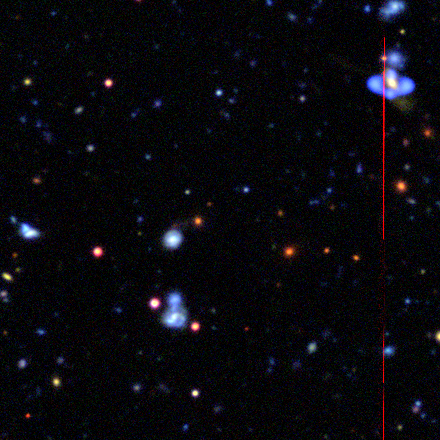
\includegraphics[trim = 128mm 116mm 8mm 14mm, clip, width=3cm]{Bilder/lol}%www.en.wikibooks.org/LaTeX/Importing_Graphics
\end{figure}
\newpage Nachdem ich mit dem Betrachten dieser Bildmasse fertig war, habe ich angefangen einige Simulationen mit SpaghettiLens unter die Lupe zu nehmen.
So kann man versuchen, die blauen Punkte der Gravitationslinsen, Minimas und Sattelpunkten zuzuordnen.
(Der maximale Weg geht immer gerade durch die Galaxie und ist daher nicht wahrnehmbar.)
Mit SpaghettiLens kann man dann ueberpruefen, ob die Zuordnung sinnvoll ist oder ob eine andere Konstellation der Punkte sinnvoller waere.
Sobald man eine sinnvolle Zusammenstellung entdeckt hat, kann man die Masseverteilung der vorderen Galaxie, wie auch einige weitere Informationen herauslesen.
Hier eine von mir bearbeitete Linse:
%todo An dieser Stelle noch ein Beispiel fuer eine Bearbeitete Linse...


\paragraph{Beispiel (ASW0001a8c):}
http://mite.physik.uzh.ch/data/002980

\begin{figure}[position=h]
\centering
 \caption{In das Programm eingespreiste Information:\newline
  (rot = Maxima, blau = Minima, gruen = Sattelpunkt)}
 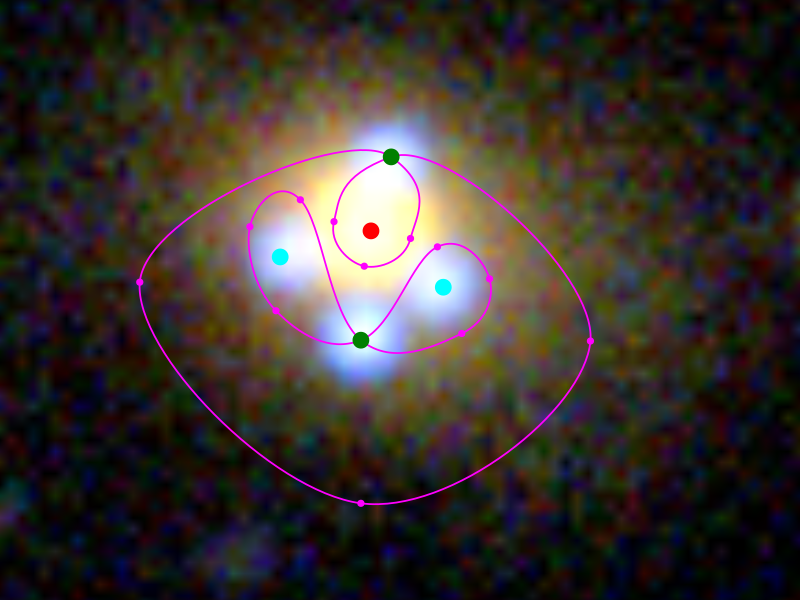
\includegraphics[trim = 40mm 50mm 60mm 40mm, clip, width=8cm]{Bilder/workinput}%www.en.wikibooks.org/LaTeX/Importing_Graphics
\end{figure}

\begin{figure}[position=h]
\centering
 \caption{Masseverteilung:}
 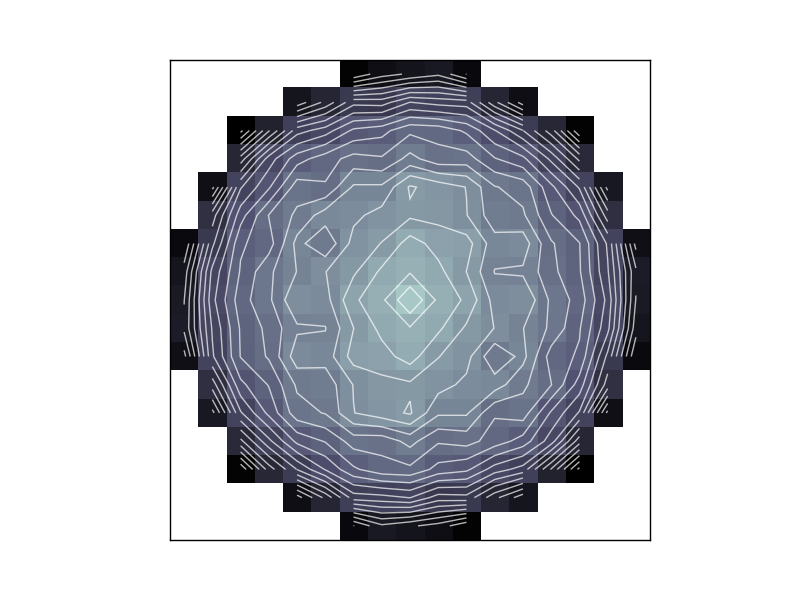
\includegraphics[width=10cm]{Bilder/workoutput3}%www.en.wikibooks.org/LaTeX/Importing_Graphics
\end{figure}

\begin{figure}[position=h]
\centering
 \caption{Empfangenes Licht mit der Verteilung der Simulation:\newline
  (Desto dunkler, desto hoehere Photonendichte)}
 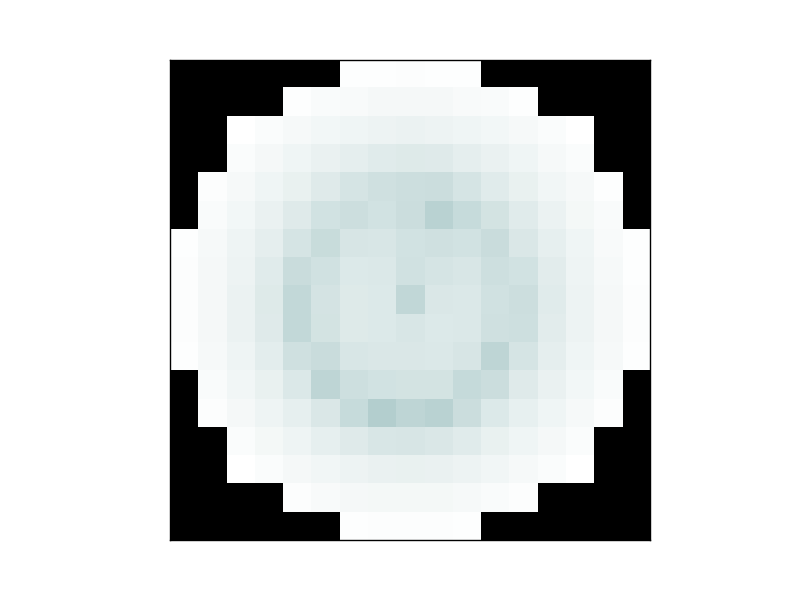
\includegraphics[width=10cm]{Bilder/workoutput2}%www.en.wikibooks.org/LaTeX/Importing_Graphics
\end{figure}

\begin{figure}[position=h]
\centering
 \caption{Minimas, Maxima, Sattelpunkte:}
 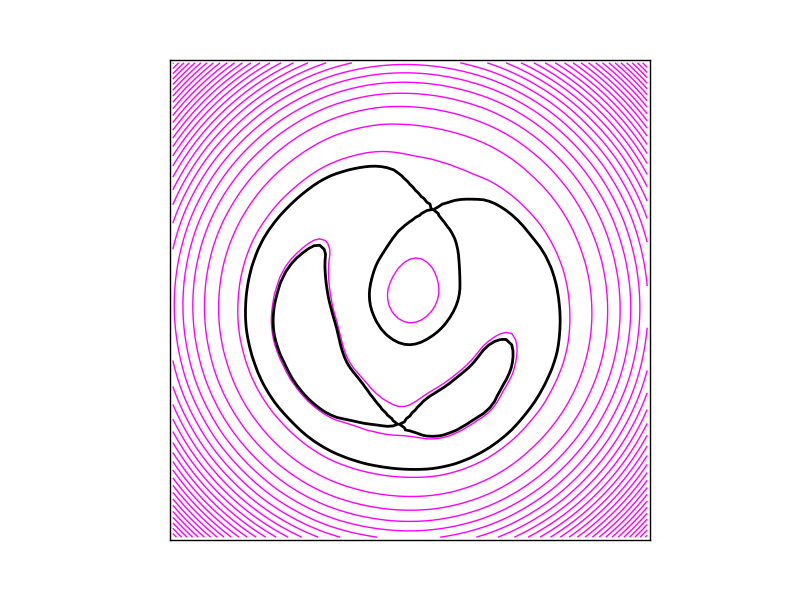
\includegraphics[width=10cm]{Bilder/workoutput1}%www.en.wikibooks.org/LaTeX/Importing_Graphics
\end{figure}

\newpage

\section {Laplace}

Danach habe ich mit dem Programmieren des Laplace Problemes begonnen.
Dazu habe ich zuerst eine vereinfachte Version programmiert.

\subsection {Uebung zum Programmieren}

Im einfacheren Problem geht es darum, die genauen Punkte einer moeglichst kleinen Flaeche zu berechnen.
Dies machen wir mit der an der Kantonsschule behandelten Programmiersprache Python.
Stellen sie sich ein Rechteck aus Draht vor.
Nun verbiegen sie es etwas, so dass es von oben betrachtet wie ein Rechteck,
von der Seite jedoch uneben ist.
Geben sie diesen Draht in etwas Seifenblasenwasser. 
Die Flaeche der innerhalb des Rechtecks entstandenen Seifenblase versucht sich moeglichst klein zu halten. 
Genau fuer diese Flaeche habe ich ein Programm geschrieben, welches jeden beliebigen Punkt der Oberflaeche mit Hilfe der Topografie der Drahtraender errechnen kann.
Die Berechnung fuer diese Flaeche erfolgt durch das wiederholte Ersetzen der Punkte durch den Durchschnitt der umliegenden Punkte bis die Aenderung des Punktes durch die wiederholte Rechnung gegen Null sinkt.

\newpage
\paragraph {Python}

Das Herzstueck meines ersten Programmtypes, welcher die neuen Punkte berechnet:

\begin{lstlisting}
# Parameter

h = 0
i = 20 # gewuenschte Anzahl X-Werte
j = 20 # gewuenschte Anzahl Y-Werte
z = 0.01 #gewuenschte Maximalabweichung (absolut)

# Erstellen einer Liste k

m = range(0, j)
l = []
k = []
for i in range(i):
  l.append(m)
k.append(l)

# Start der Berechnungen

while z*((i - 2)*(j - 2)) < r :
    
    h += 1

    # Fuer jede Berechnungstiefe wird ein neues
    # Listenelement erzeugt und hinzugefuegt.

    for a in range(0, i):
        for b in range(0, j):
            e = k[h - 1][a][b]
            u.append(e)
        v.append(u)
    k.append(v)

    # Hier werden die neuen Punkte errechnet

    for a in range(1, i - 1):
        for b in range(1, j - 1):
            k[h][a][b] = (k[h-1][a+1][b] \
+ k[h-1][a-1][b] + k[h-1][a][b+1] \
+ k[h-1][a][b-1]) / 4

    # In diesem Bereich wird geprueft, ob die 
    # gewuenschte Genauigkeit bereits erreicht wurde.

    r = 0
    for a in range(1, i - 1):
        for b in range(1, j - 1):
            e = (k[h][a+1][b] + k[h][a-1][b] \
+ k[h][a][b+1] + k[h][a][b-1]) / 4
            f = (e-k[h][a][b])*(e-k[h][a][b])
            #print("Tiefe:", h, "X-Achse:", a, \
"Y-Achse:", b, "Hoehe:" , k[h][a][b], \
"Abweichung:", f)
            if f <= z:
                r += f
            else:
                r = p*i*j
\end{lstlisting}

\subsection {Laplace - Poisson}

Fuer das echte Laplace Problem habe ich den Rand auf Null gesetzt und in der Mitte die Berechnung einiger Punkte etwas komplizierter gestaltet.
Die meisten Punkte werden immer noch durch den Durchschnitt der umliegenden Punkte errechnet.
Dort wo sich im Model eine Masse befindet, wird die Gleichung etwas angepasst und durch eine Konstante und die Abstaende der Punkte zueinander ergaenzt.
Komplexere Berechnung (dargestellt ohne Tiefenverzeichnis 'h'):
\begin{lstlisting}
z[i][j] = (z[i+1][j] + z[i-1][j] + z[i][j+1] \
+ z[i][j-1] + k*delta**2)/4  
\end{lstlisting}
Wobei 'delta' dem Abstand zwischen den Punkten entspricht. Stellt man diese Punkte dreidimensional dar, so entsteht das typische Bild von diesem Algorithmus, von welchem es zahlreiche Bilder im Internet gibt.
Fertig ist die Berechnung der Raumkruemmung.
Da meine Programmierkentnisse nicht ausserordentlich gross sind, habe ich viele Programmierschritte durch einfache Befehle geschrieben.
Dies hatte unweigerlich die Verlangsamung und die extreme Groesse des Programmes zur Folge.
Nachdem ich in weitere Pythonbefehle instruiert wurde, konnte ich das Programm bis auf etwa 50 Zeilen kuerzen und extrem viel schneller machen.
(Die komplexeste Version hatte \textgreater250 Zeilen.)
Dafuer habe ich viele Parameter entfernt und nur noch das Grundgeruest gelassen.
Mein Programm waere eigentlich noch kuerzer. Jedoch musste ich eine Maske definieren.
Diese hat die Eigenschaft, dass sie alle Punkte in einem gewissen Abstand zum Zentrum auf 0 setzt, um das verzerren der Berechnungen durch allfaellige Ecken zu verhindern.
Nachdem die Programmierung fertig war, habe ich sie in das abschliessende Programm eingefuegt und meine Arbeit beendet.
Unter www.github.com/Eraster/Laplace
ist es moeglich auf meine Programme zuzugreifen, wobei die komplexeste Version 
Laplace original all in one.py 
und die kuerzeste
Laplace funktion.py
heisst.


\paragraph {Funktion: Laplace (Pythonxy)}

Hier noch das Abschlussprogramm Laplace funktion.py
\begin{lstlisting}
from numpy import zeros, amax, amin
import numpy as np

def Mask(c):
    
    a = 0*c
    len = np.alen(a)
    l = float(len)
    
    dk = (l-1)/2-0.01
    
    for i in range(0, len):
        for j in range(0, len):
            dx = ((l-1)/2-i)**2
            dy = ((l-1)/2-j)**2
            dis = sqrt(dx+dy)
            
            if dis < dk:
                a[i][j] = 1
            else:
                a[i][j] = 0

def Laplace(m):
    # m == array mit Massenverteilung

    # Einstellen der Parameter

    Genauigkeit = 0.001
    z = np.abs(Genauigkeit)
    delta = 2
    repeat = 10000
    
    mas = Mask(m)
    
    konstant = ((1*m)*delta**2)/4
    kd = 0*m
    k = []
    k.append(kd)
    
    h = 0
    r = z + 1

    while z < r and repeat > h :

	# Berechnung der neuen Tiefe + 
	# neues Listenelement + Pruefung
        
        h += 1
        kd = k[h - 1]
        average = 1*kd
        average[1:-1, 1:-1] = (kd[0: -2, 1: -1] \
+ kd[2:, 1: -1] \
+ kd[1: -1, 0: -2] + kd[1: -1, 2:])/4
        kd = (average + konstant)*mas
        k.append(kd)
    
        if amax(k[h] - k[h-1]) <= z and amin(k[h] \
- k[h-1]) >= -1*z:
            r = 0
        else:
            r = z + 1
                
    return kd
\end{lstlisting}

\newpage

\section{Lensing}

(Es tut mir leid, diesen Text nicht auch in Deutsch verfasst zu haben. Ich bitte vielmals um Entschuldigung. Dieser Text wurde in Englisch verfasst, da wir in in Englisch verwenden werden (zooniverse).
\\[3mm]
In this part of my little article, I will give you a closer look on my calculation (fermat and laplace). First of all, the calculation itself isn`t very difficult but the theorie behind is. So what I will do is just describing the Laplace- and Farmacalculation. In the end, you will recognize the sattlepoints, the minimas and the maximum and know their meaning. But you won`t understand the rason why it is this way! 

\subsection{Laplace}

The first part of the calculation is to solve the Laplace-problem for the mass you have. (It is simple to work with a big mass in the very center of your map.) The goal is that every point on your mass profile fulfills its definition. For the perfect calculation, every Point of the surface comes true with this formula:


\[                                                            
	\text{average}\cdot\frac{\text{mass}\cdot\Delta}{4}- \text{value}= 0
\]
average: Average of the points around the point you`re looking at.
\\[0mm]
delta: distance between your measurements
\\[0mm]
mass: Thats the most important part! For nice programming this should be an array with 2 Dimensions. Every Point has his specific mass.
\\[0mm]
value: Value of the point you`re looking at.
\\[3mm]
After this calculation you don`t have a mass profile anymore, but the map of a kind of space curvature. Because we calculate with numeric systems, in most cases it`s impossible to reach the absolute correct solution. (That means that the computer will stay in a loop if you program it to give you the perfect solution.) An approximation is required. I programmed this calculation with a loop. The loop replaces the value of every point by this calculation:

\[                                                            
	\text{Laplace(point) :}= \text{average}\cdot\frac{\text{mass}\cdot\Delta}{4}
\]

The loop goes as long, as the approximation isn`t good enough. (You can have a look at this on the funciton: Laplace (Pythonxy) from this article.

\begin{figure}[position=h]
\centering
 \caption{space curvature (matplot)}
 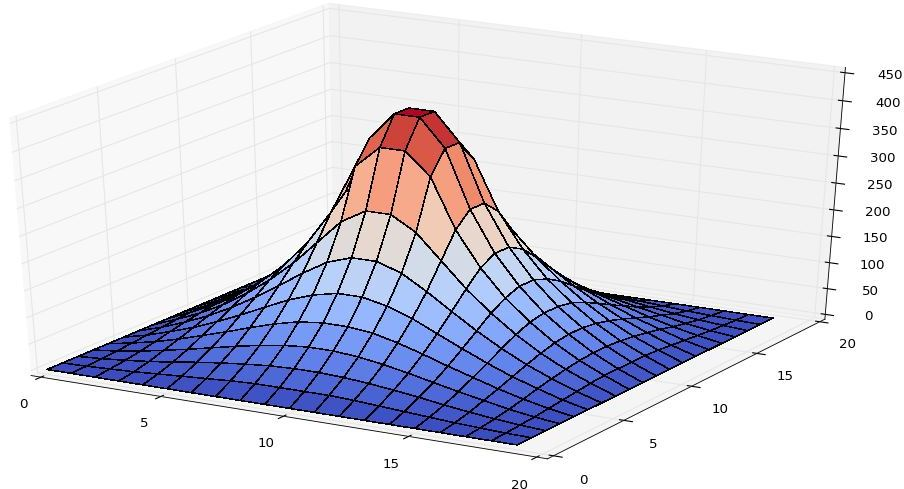
\includegraphics[width=10cm]{Bilder/Laplace}%www.en.wikibooks.org/LaTeX/Importing_Graphics
\end{figure}


\subsection{Fermatprinzip}

As a second step, we have to add a value to the solution from Laplace to get the solution for the fermat law.
The value which we add is definied as the distance to the centre in square. The center is a definied point in the middle of the calculation.

\[                                                            
	Ferma(point):= \text{k}\cdot\left(x^2\cdot\ y^2\right) + \text{Laplace(point)}
\]

k: difficult konstant (I havent worked with it yet but for qualitative right results just set it to 1.)

\(x^2 \cdot y^2 \): This is just the distance to the middle point in square.
\\[3mm]
If you have calculatet that its easy to animate it. I just did it with matplot and it looked like this:

\begin{figure}[position=h]
\centering
 \caption{Distance in square}
 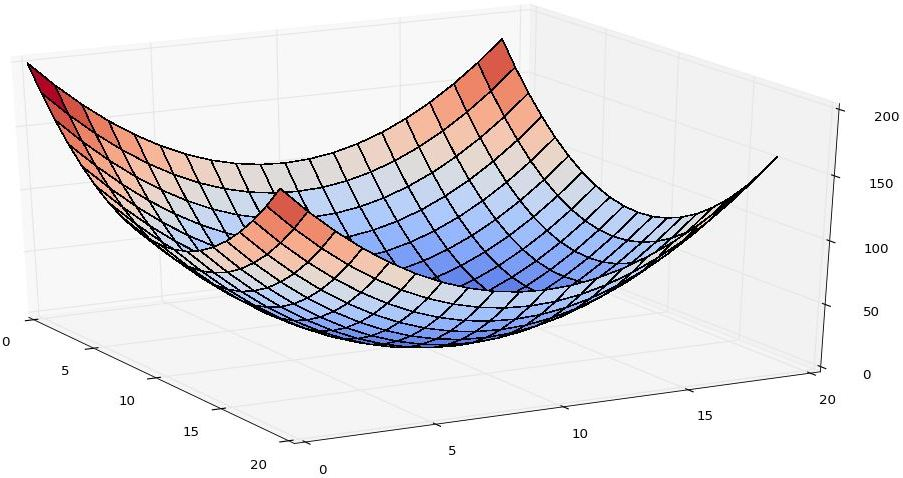
\includegraphics[width=10cm]{Bilder/xxyy}%www.en.wikibooks.org/LaTeX/Importing_Graphics
\end{figure}

\newpage

Here you see the calculation(distance in square + Laplace):
\\[0mm]
h: This is the calculated array.


\begin{lstlisting}
import numpy as np
from matplotlib import cm
from mpl_toolkits.mplot3d.axes3d import get_test_data
import matplotlib.pyplot as plt

# Twice as wide as it is tall.
fig = plt.figure()

#---- First subplot
ax = fig.add_subplot(1, 1, 1, projection='3d')
#ax.set_zlim(1500,3000)

X = np.arange(0, 100, 1)
Y = np.arange(0, 100, 1)
X, Y = np.meshgrid(X, Y)

plt.axis('equal')

surf = plt.contour(X, Y, h, 75,rstride=1, \
 cstride=1, cmap=cm.coolwarm, \
 linewidth=0.1, antialiased=False)

#---- Second subplot

plt.show()

\end{lstlisting}

In the appendix you find the whole program for my fermat calculation. (It`s the shortest version I have from this sort of calculation.)

\subsection{Usage}

As soon as the calculation is complete. You can see the sattlepoints who look like an "8". Maximas are just the highest spots and minimas the pits. It should look like that:

\begin{figure}[position=h]
\centering
 \caption{2D Fermat (simple)}
 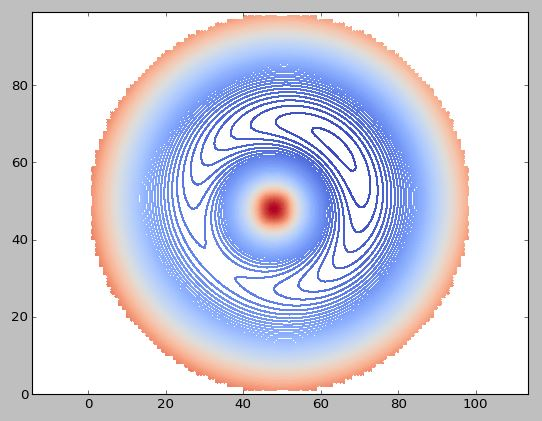
\includegraphics[width=10cm]{Bilder/simpl}%www.en.wikibooks.org/LaTeX/Importing_Graphics
\end{figure}

\clearfloat

In Spaghettilens the imput is just a map with these 3 kinds of points. The goal is then to calculate this vice versa. So what Spaghettilens does is just the calculation I explained the other way round. Because this is difficult and you can`t find the absolute true solution. In the project you give some Citizen Scientists pictures from spacewarps like this:

\begin{figure}[position=h]
\centering
 \caption{Input}
 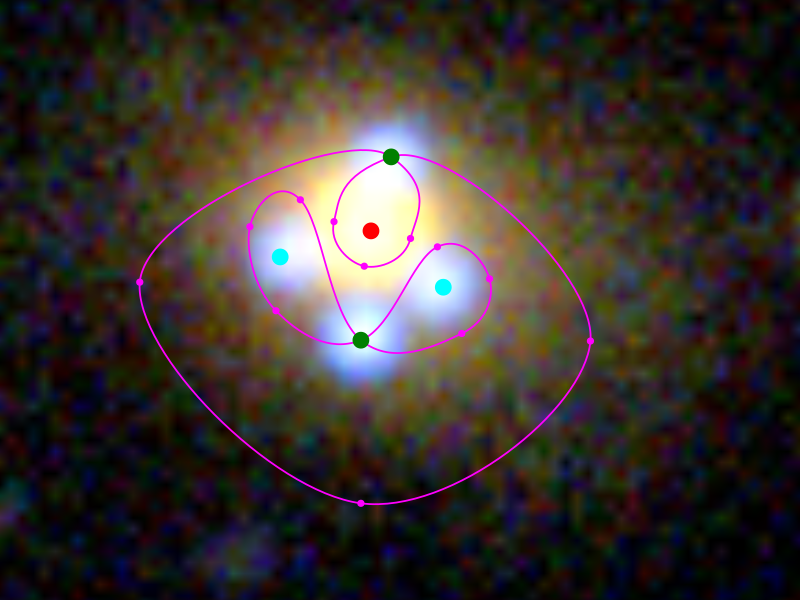
\includegraphics[width=10cm]{Bilder/workinput}%www.en.wikibooks.org/LaTeX/Importing_Graphics
\end{figure}

\clearfloat
http://mite.physik.uzh.ch/data/002996
\\[0mm]
They then mark these 3 kinds of points (red = maximum, blue = minimum, green = sattlepoint) and the calculation can run. First we tried this with simulated lenses and looked how close the Citizen Scientists come to the solution. We found out, that if the mass is centered, they manage to mark everything right. Becuase then you only see 1 maximum, minimum and sattlepoint. But if the mass gets more complicated there aren`t just 3 spots anymore. In most of these cases, there are 2 sattlepoints, 2 minimas and 1 maxima. In this case, there often are some difficulties to put them on the right place. This work really is important because there is no way to write an algorithm yet who manages to do this work. The findings are then looked at and may pull us a bit further in science. I wish all of these scientists good look because my time here is over. Good Luck and good bye.

\begin{figure}[position=h]
\centering
 \caption{2D Fermat}
 \includegraphics[width=10cm]{Bilder/Fermat2}%www.en.wikibooks.org/LaTeX/Importing_Graphics
\end{figure}

\begin{figure}[position=h]
\centering
 \caption{3D Fermat}
 \includegraphics[width=15cm]{Bilder/Fermat}%www.en.wikibooks.org/LaTeX/Importing_Graphics
\end{figure}

\clearpage
\section{Fazit}
In meinem Praktikum habe ich im Bereich meiner Moeglichkeiten so gut es geht mitgearbeitet.
Schlussendlich konnte ich die Laplacefunktion einbauen und bin sehr stolz darauf.
Solch ein Praktikum bietet einen besonderen Einblick in das Leben und die Arbeitsweise an der Universitaet Zuerich.
Es ist mir daher eine Ehre, hier arbeiten zu duerfen.
Das alles waere nicht moeglich gewesen ohne die grosse Unterstuetzung von Rafael Kueng, Doktor Prasenjit Saha und Professor Doktor Thomas Gehrmann,
welcher es mir erst ermoeglichte, mein Praktikum hier an der UZH zu starten.
Zum Abschluss moechte ich Ihnen ganz herzlich danken.

\newpage
\section{Appendix}

\begin{lstlisting}
from numpy import zeros, amax, amin
import numpy as np
import numpy as np
from matplotlib import cm
from mpl_toolkits.mplot3d.axes3d import get_test_data
import matplotlib.pyplot as plt

def Mask_a(c):
    
    a = 0*c
    len = np.alen(a)
    l = float(len)
    
    dk = (l-1)/2-0.01
    
    for i in range(0, len):
        for j in range(0, len):
            dx = ((l-1)/2-i)**2
            dy = ((l-1)/2-j)**2
            dis = np.sqrt(dx+dy)
            
            if dis < dk:
                a[i][j] = 1
            else:
                a[i][j] = 0
                
    return a

def Laplace(m):
    
    Genauigkeit = 0.001
    z = np.abs(Genauigkeit)    
    delta = 2    
    repeat = 10000
    
    mas = Mask_a(m)
    
    konstant = ((1*m)*delta**2)/4    
    kd = 0*m
    k = []
    k.append(kd)
    
    h = 0        
    r = z + 1

    while z < r and repeat > h :
        
        h += 1        
        kd = k[h - 1]
        average = 1*kd
        average[1:-1, 1:-1] = (kd[0: -2, 1: -1] \
				+ kd[2:, 1: -1] + kd[1: -1, 0: -2] \
				+ kd[1: -1, 2:])/4
        kd = (average + konstant)*mas
        k.append(kd)
    
        if  amax(k[h] - k[h-1]) <= z  \
				and amin(k[h] - k[h-1]) >= -1*z:
            r = 0                
        else:
            r = z + 1
                
    return kd
    
def Fermat(m):
    
    place = Laplace(m)
    xlen = float(len(place))
    ylen = float(len(place))
    xy = 0*place
    
    
    for i in range(len(place)):
        for j in range(len(place[0])):
            xy[i][j] = (xlen/2-i)**2+(ylen/2-j)**2
						# factor k == 1
		
    ferma = place + xy
    
    return ferma
    
def Mask_b(c):
    
    a = c
    len = np.alen(a)
    l = float(len)
    
    dk = (l-1)/2-0.01
    
    for i in range(0, len):
        for j in range(0, len):
            dx = ((l-1)/2-i)**2
            dy = ((l-1)/2-j)**2
            dis = sqrt(dx+dy)
            
            if dis < dk:
                pass
            else:
                a[i][j] = None
                
    return a    
    
    
ma = zeros((100,100), float)

ma[45: 50, 30: 70] = 10#ma[45: 50, 30: 70] = 10
        
h = Fermat(ma)
h = Mask_b(h)

# Animation

# Twice as wide as it is tall.
fig = plt.figure()

#---- First subplot
ax = fig.add_subplot(1, 1, 1, projection='3d')
#ax.set_zlim(1500,3000)

X = np.arange(0, 100, 1)
Y = np.arange(0, 100, 1)
X, Y = np.meshgrid(X, Y)

plt.axis('equal')

surf = plt.contour(X, Y, h, 75,rstride=1, \
 cstride=1, cmap=cm.coolwarm, \
 linewidth=0.1, antialiased=False)

#---- Second subplot

plt.show()




\end{lstlisting}


\end{document}

